\documentclass{beamer}
\mode<presentation>
{
  \usetheme{Warsaw}
  \definecolor{mcgarnet}{rgb}{0.38, 0, 0.08}
  \definecolor{mcgray}{rgb}{0.6, 0.6, 0.6}
  \setbeamercolor{structure}{fg=mcgarnet,bg=mcgray}
  %\setbeamercovered{transparent}
}


\usepackage[english]{babel}
\usepackage[latin1]{inputenc}
\usepackage{times}
\usepackage[T1]{fontenc}
\usepackage{tikz}
\usepackage{graphicx}
\usepackage{amsmath}
\usepackage{multirow}

\newcommand{\imagesource}[1]{{\centering\hfill\break\hbox{\scriptsize Image Source:\thinspace{\small\itshape #1}}\par}}

\title{Lecture 1 - Numbers and Notation}


\author{Robert Lowe\\}

\institute[Maryville College] % (optional, but mostly needed)
{
  Division of Mathematics and Computer Science\\
  Maryville College
}

\date[]{}
\subject{MTH110 - Quantitative Literacy}

\pgfdeclareimage[height=0.5cm]{university-logo}{images/Maryville-College}
\logo{\pgfuseimage{university-logo}}



\AtBeginSection[]
{
  \begin{frame}<beamer>{Outline}
    \tableofcontents[currentsection]
  \end{frame}
}


\begin{document}

\begin{frame}
  \titlepage
\end{frame}

\begin{frame}{Outline}
  \tableofcontents
\end{frame}


% Structuring a talk is a difficult task and the following structure
% may not be suitable. Here are some rules that apply for this
% solution: 
%
% - Exactly two or three sections (other than the summary).
% - At *most* three subsections per section.
% - Talk about 30s to 2min per frame. So there should be between about
%   15 and 30 frames, all told.
%
% - A conference audience is likely to know very little of what you
%   are going to talk about. So *simplify*!
% - In a 20min talk, getting the main ideas across is hard
%   enough. Leave out details, even if it means being less precise than
%   you think necessary.
% - If you omit details that are vital to the proof/implementation,
%   just say so once. Everybody will be happy with that.

\section{Quantitative Language}

\begin{frame}{Why You Are Bad at Math}

\begin{itemize}[<+(1)->]
    \item You have been taught a litany of rules and procedures, but no ideas.
    \item Your textbooks were lacking in text.  Lots of color, lots of problems, no substance!
    \item Being bad at math was socially acceptable, and you seized the opportunity because memorizing rules and procedures is boring.
\end{itemize}

\end{frame}


\begin{frame}{A Brief History of Counting}
\begin{itemize}[<+(1)->]
    \item Tally Marks 40,000 years old 
    \item Ishango Bone 20,000 years old, may have been a rudimentary calculator
    \item Formal mathematics, as we know it today, really started about 3000 years ago
\end{itemize}
\end{frame}

\begin{frame}{Ancient Numeral Systems - Roman Numerals}
\begin{itemize}[<+(1)->]
    \item Representing Numbers as Figures
    \item Example: Roman Numeral System
    
    \begin{tabular}{|lr|lr|}
    \hline
    \multicolumn{2}{|c|}{Numerals} & \multicolumn{2}{|c|}{Transitions} \\
    \hline
    I & 1 & &\\
    V & 5 & IV & 4\\
    X & 10 & IX & 9\\
    L & 50 & XL & 40 \\
    C & 100 & XC & 90\\
    D & 500 & CD & 400\\ 
    M & 100 & CM & 900\\
    \hline
    \end{tabular}
\end{itemize}
\end{frame}

\begin{frame}
\begin{itemize}[<+(1)->]
    \item Arithmetic was usually done with some sort of manipulative aid (counting board, abacus, etc).
    \item Roman numeral arithmetic is difficult. (Let's Try it)
    \begin{enumerate}
        \item $\mathrm{I}\ +\ \mathrm{I}=?$
        \item $\mathrm{III}\ +\ \mathrm{I}=?$
        \item $\mathrm{XV}\ -\ \mathrm{V}=?$
        \item $\mathrm{V}\ -\ \mathrm{I}=?$
        \item $\mathrm{V}\ \times\ \mathrm{IV}=?$
    \end{enumerate}
\end{itemize}
\end{frame}

\begin{frame}{The Arabic/Indian Numeral System}
\begin{columns}
\column{0.6\textwidth}
\begin{itemize}[<+(1)->]
    \item Introduced to the Western world by Al-Khwarizmi, but was invented in India
    \item Digits 0-9
    \item Positional value system
    \[
    \begin{array}{|l|l|l|l|}
        & & & \\
        \hline
        10^3 & 10^2 & 10^1 & 10^0\\
        \hline
    \end{array}
    \]
\end{itemize}

\column{0.4\textwidth}

\includegraphics[width=0.9\textwidth]{images/Al-Khwarizmi}
{\tiny Image Source:
\newline \url{https://www.mathematics-monster.com/glossary/Al-Khwarizmi.html}}
\end{columns}

\end{frame}


\begin{frame}{The Arabic/Indian Numeral System}
\begin{columns}
\column{0.6\textwidth}
\begin{itemize}[<+(3)->]
    \item Works very well for arithmetic!
    \begin{enumerate}
        \item $1+1=?$
        \item $3+1=?$
        \item $15+5=?$
        \item $5-1=?$
        \item $5\times 4=?$
    \end{enumerate}
\end{itemize}

\column{0.4\textwidth}
\uncover<2->{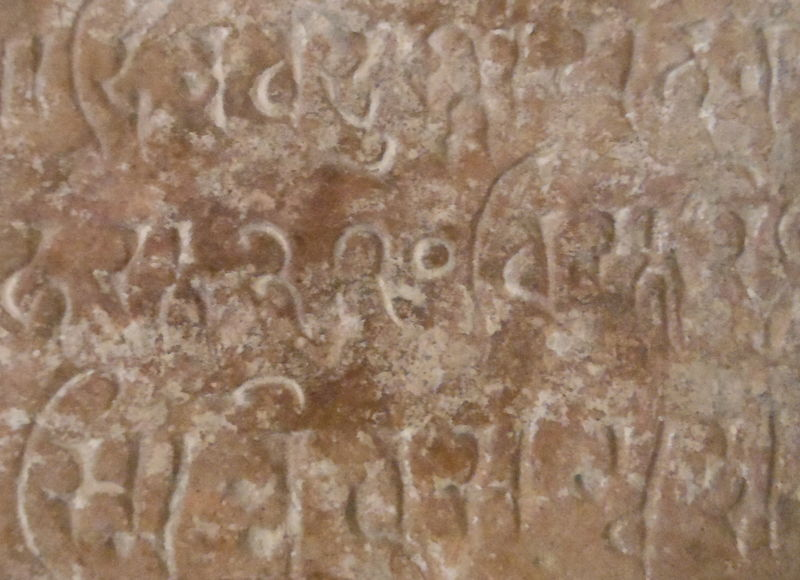
\includegraphics[height=0.35\textheight]{images/zero}}
\newline
\uncover<3->{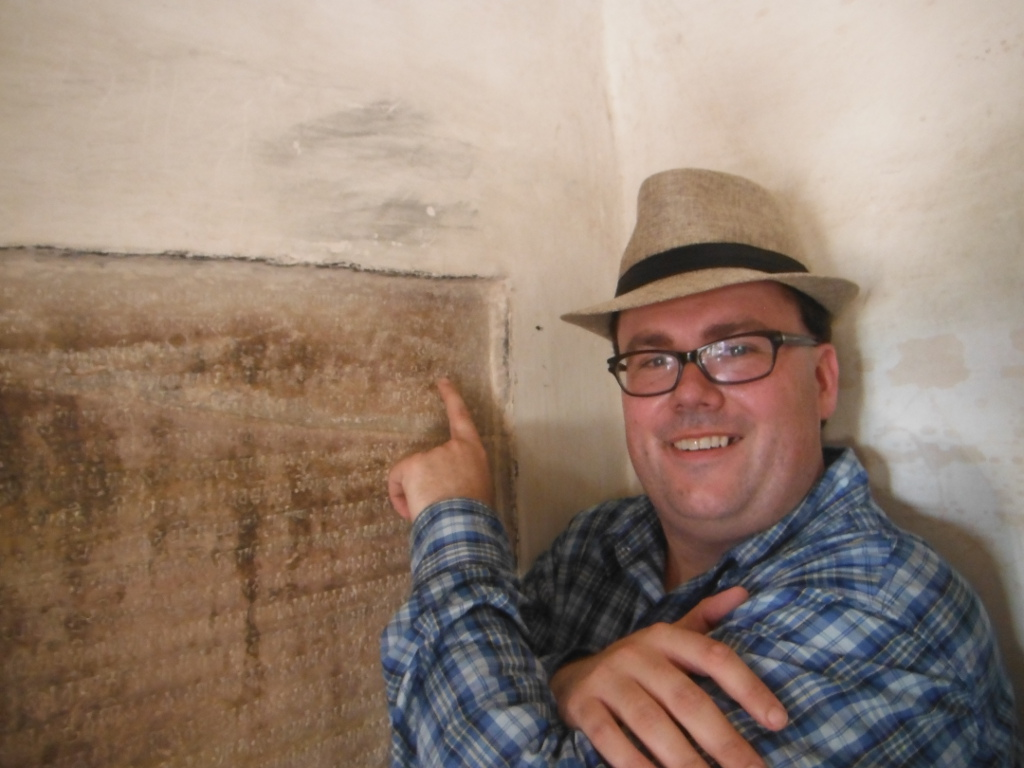
\includegraphics[height=0.35\textheight]{images/me-zero}}
\end{columns}

\end{frame}

%%%%%%%%%%%%%%%%%%%%%%%%%%%%%%%%%%%%%%%%%%%%%%%%%%%%%%%%%%%%%%%%%%%%%%
\section{Evaluating Expressions}

\begin{frame}{Fundamental Operations of Arithmetic}
\begin{itemize}[<+(1)->]
    \item Fundamental operations: $+$, $-$, $\times$, $\div$
    \item Alternate notations for multiplication: $3\times 5$, $3\cdot 5$, $3(5)$, $3*5$
    \item Alternate notations for division: $4\div 2$, $\frac{4}{2}$, $2\overline{)4}$, $4/2$
\end{itemize}
\end{frame}

\begin{frame}{Order of Operations and Reduction}
\begin{itemize}[<+(1)->]
    \item Convention PEMDAS - Parenthesis, Exponent, Multiply, Divide, Add, Subtract
    \item Multiplication and Division are the same operation, so is Add and Subtract \newline
    \begin{tabular}{llllll}
        \multirow{2}{*}{P} & \multirow{2}{*}{E} & M & A\\
        & & D & S\\
    \end{tabular}\newline
    Ties are broken left to right
    \item Example: $3^2+4\times2-16\div(2+2)$
\end{itemize}
\end{frame}

\begin{frame}{Scientific Notation}
\begin{itemize}[<+(1)->]
    \item Writing very large or very small numbers is very error prone.
    \item We usually only really care about the first few values (more on this later).
    \item Base 10 gives us a way to do this!
    \item Large numbers have 0's at the right hand side.  This is effectively multiplying
    by 10.  So we can use exponents:
    \[
    1,200,000 = 1.2 \times 10^6
    \] 
   \item Small numbers of 0's between the decimal point and nonzero digits.  This is effectively dividing by 10:
   \[
   0.0000012 = 1.2 \times 10^{-6}
   \]
\end{itemize}
\end{frame}
\end{document}

